%!TEX root = ../doc.tex
\documentclass[../doc.tex]{subfiles}

\begin{document}
\chapter{Second Moment Methods} \label{chap:smm}
Lewis and Miller's \gls{smm} \cite{lewis_miller} couples the transport equation to the moment equations with additive closures that depend linearly on the transport solution. This scheme is characterized by a two-stage process where 1) the transport equation is inverted with a scattering source defined from the previous iteration's SMM scalar flux and 2) a \emph{diffusion approximation} is solved with transport-dependent correction sources. By contrast, VEF uses nonlinear closures and the generally non-symmetric VEF moment system must be solved at each iteration. Since SMM solves the symetric diffusion equation instead of the non-symmetric VEF equations, less expensive solvers, such as conjugate gradient, can be used instead of the general purpose methods such as \gls{bicg} or \gls{gmres} which generally require more computation and storage. 
In addition, where the VEF closures are well defined only when $\psi>0$, the additive closures used in SMM are well-defined for any $\psi$. 

Here, we pursue independent discretizations of the SMM moment system. 
An independent method can be designed such that its diffusion system exactly matches that of an existing radiation diffusion package. The existing diffusion package could then be extended to a transport algorithm by simply supplying a modified, transport-dependent source term corresponding to the SMM correction sources. Such a method would ease code coupling between radiation and hydrodynamics and allow reuse of the existing linear and nonlinear solvers implemented for radiation diffusion. Finally, the independent approach allows the moment system to be agnostic to the transport solver. For example, the correction sources could be computed using a stochastic solver such as \gls{imc}. 

We note that, since the left hand side of the SMM moment system is simply radiation diffusion, consistent SMMs can be designed by using any of the diffusion discretizations developed for consistent \gls{dsa} methods such as \textcite{WWM,AM,WR,ldrd_dsa}. Furthermore, many consistent DSA schemes can be scalably solved with preconditioned iterative solvers (e.g.~\cite{ldrd_dsa,WR}). The design of efficient, consistent SMM algorithms then only requires developing consistent discretizations for the SMM correction sources. Thus, in the case of SMM, the consistent approach is likely to be effective. However, such a method would not enjoy the flexibilities discussed above. 

In this chapter, we use the connection between VEF and SMM established in Section \ref{moment_sec:linearize} to derive discrete SMMs. This connection provides a systematic path to deriving discrete SMMs from existing VEF methods. In particular, we derive SMM analogs of the interior penalty, continuous finite element, and mixed finite element methods presented in Chapters \ref{chap:dgvef} and \ref{chap:rtvef}. The chapter concludes with numerical results demonstrating the accuracy and performance of the methods. 

\section{Discrete Second Moment Methods}
The equivalence of SMM and VEF linearized about a linearly anisotropic solution provides a systematic path toward deriving discrete SMMs. Any VEF method can be converted to an SMM through the linearization process described in Section \ref{moment_sec:linearize}. We make use of the structure of the coupled transport-VEF system to simplify the derivations. Consider
	\begin{equation}
		\F(\psi,\mat{X}) = \begin{bmatrix} 
			\mat{\Theta}(\psi,\varphi) \\ \mat{V}(\psi,\mat{X}) 
		\end{bmatrix} = 0\,,
	\end{equation}
where $\mat{\Theta}(\psi,\varphi)$ represents a generic transport discretization and $\mat{V}(\psi,\varphi)$ a generic discretization of the VEF moment equations. The moment system's unknowns are represented by $\mat{X}$ which includes the scalar flux and current for discretizations of the first-order form of the VEF equations and just the scalar flux for discretizations in second-order form. 
Here, $\mat{\Theta}$ and $\mat{V}$ include the inflow and Miften-Larsen boundary conditions, respectively. 
Given that the operators that make up the discretization of the transport equation are linear in both the angular and scalar flux and that the operators in the VEF discretization are nonlinear in the angular flux and linear in the scalar flux (and current where applicable), the linearization process will produce a system of the form: 
	\begin{equation}
		\begin{bmatrix} 
			\mat{\Theta}(\psi,\varphi) \\
			\displaystyle\mat{V}(\psi_0,\mat{X}) + \pderiv{\mat{V}}{\psi}\biggr\rvert_{\psi_0}
		\end{bmatrix} = 0 \,, 
	\end{equation}
where $\psi_0$ is the diffusion approximation of the transport problem. 
In other words, we have the original transport equation coupled to a discretization of diffusion with a $\psi$-dependent correction term arising from the derivative of the VEF operator, $\pderiv{\mat{V}}{\psi}$, evaluated at the diffusion approximation to the transport problem. 

In the following subsections, the methods derived in Chapters \ref{chap:dgvef} and \ref{chap:rtvef} are linearized to form discrete SMMs by determining 1) the diffusion problem, $\mat{V}(\psi_0, \mat{X})$, found by evaluating the VEF system using a linearly anisotropic angular flux and 2) the transport-dependent correction terms corresponding to $\pderiv{\mat{V}}{\psi}\big\rvert_{\psi_0}$. We will see that linearizing the \emph{discrete} VEF system provides a straightforward path toward discretizing the correction terms. 

\subsection{Interior Penalty}
From Section \ref{dgvef_sec:ip}, the IP VEF discretization is: find $\varphi\in Y_p$ such that 
	\begin{multline} \label{smm:ipvef}
		\int_{\Gamma_b} E_b\, u \varphi \ud s + \int_{\Gamma_0} \kappa \jump{u} \jump{\varphi} \ud s - \int_{\Gamma_0} \jump{u} \avg{\frac{1}{\sigma_t}\nablah\cdot\paren{\E\varphi}\cdot\n} \ud s - \int_{\Gamma_0} \avg{\frac{\nablah u}{\sigma_t}} \cdot \jump{\E\varphi\n} \ud s \\
		+ \int \nablah u \cdot \frac{1}{\sigma_t}\nablah\cdot\paren{\E\varphi} \ud \x + \int \sigma_a\, u \varphi \ud \x \\ 
		= \int u\, Q_0 \ud \x + \int \nablah u \cdot \frac{\vec{Q}_1}{\sigma_t} \ud \x - \int_{\Gamma_0} \jump{u} \avg{\frac{\vec{Q}_1\cdot\n}{\sigma_t}} \ud s - 2\int_{\Gamma_b} u\, \Jin \ud s \,, \quad \forall u \in Y_p \,, 
	\end{multline}
where $\kappa$ is the penalty parameter. Evaluating the VEF data when the angular flux is linearly anisotropic gives
	\begin{equation}
		\E = \frac{1}{3}\I \,, \quad E_b = \frac{1}{2} \,. 
	\end{equation}
The diffusion operator is then 
	\begin{multline}
		\frac{1}{2}\int_{\Gamma_b} u\varphi \ud s + \int_{\Gamma_0} \kappa\, \jump{u}\jump{\varphi} \ud s - \int_{\Gamma_0} \jump{u}\avg{D\nablah\varphi\cdot\n} \ud s - \int_{\Gamma_0} \avg{D\nablah u\cdot\n} \jump{\varphi} \ud s \\
		+ \int \nablah u \cdot D\nablah\varphi \ud \x + \int \sigma_a\, u \varphi \ud \x \\
		= \int u\, Q_0 \ud \x + \int \nablah u \cdot \frac{\vec{Q}_1}{\sigma_t} \ud \x - \int_{\Gamma_0} \jump{u} \avg{\frac{\vec{Q}_1\cdot\n}{\sigma_t}} \ud s - 2\int_{\Gamma_b} u\, \Jin \ud s \,,
	\end{multline}
where $D = \frac{1}{3\sigma_t}$ is the diffusion coefficient. 

Next, we must determine the correction terms by computing the partial derivative with respect to the angular flux of each of the terms in the IP VEF discretization (Eq.~\ref{smm:ipvef}). We set the diffusion solution $\y_0 = \vector{\psi_0 & \phi_0}$. For terms without VEF data, the partial derivative is zero. Consider 
	\begin{equation}
		\pderiv{}{\psi}\int_{\Gamma_b} E_b\, u \varphi \ud s \biggr\rvert_{\y_0} = \int_{\Gamma_b} \pderiv{E_b}{\psi}\biggr\rvert_{\psi_0} \, u \varphi_0 \ud s = \int_{\Gamma_b} u\, \beta(\psi) \ud s \,, 
	\end{equation}
where $\beta(\psi)$ is the correction factor defined in Eq.~\ref{moment:corrfac}. We have used the directional derivative of the Eddington boundary factor computed in Eq.~\ref{moment:Eb_deriv} to simplify the term $\pderiv{\E}{\psi}$. 
Here, $\pderiv{\varphi}{\psi} = 0$ since we consider $\psi$ and $\varphi$ as independent variables. 
Analogously, for terms with the Eddington tensor
	\begin{equation}
		\pderiv{(\E\varphi)}{\psi}\biggr\rvert_{\y_0} = \pderiv{\E}{\psi}\biggr\rvert_{\psi_0} \varphi_0 = \T(\psi) \,,
	\end{equation}
where the directional derivative of the Eddington tensor is given by Eq.~\ref{moment:Edd_deriv} and $\T(\psi)$ is the correction tensor from Eq.~\ref{moment:corrten}. 
Thus, the correction terms can be derived by setting terms without angular flux dependence to zero and replacing 
	\begin{equation}
		E_b\varphi \rightarrow \beta(\psi) \,, \quad \E\varphi \rightarrow \T(\psi) \,. 
	\end{equation}
The IP SMM discretization is then: find $\varphi \in Y_p$ such that 
	\begin{multline}
		\frac{1}{2}\int_{\Gamma_b} u\varphi \ud s + \int_{\Gamma_0} \kappa\, \jump{u}\jump{\varphi} \ud s - \int_{\Gamma_0} \jump{u}\avg{D\nablah\varphi\cdot\n} \ud s - \int_{\Gamma_0} \avg{D\nablah u\cdot\n} \jump{\varphi} \ud s \\
		+ \int \nablah u \cdot D\nablah\varphi \ud \x + \int \sigma_a\, u \varphi \ud \x \\
		= \int u\, Q_0 \ud \x + \int \nablah u \cdot \frac{\vec{Q}_1}{\sigma_t} \ud \x - \int_{\Gamma_0} \jump{u} \avg{\frac{\vec{Q}_1\cdot\n}{\sigma_t}} \ud s - \int_{\Gamma_b} u\paren{2\Jin + \beta} \ud s \\
		+ \int_{\Gamma_0} \jump{u}\avg{\frac{1}{\sigma_t}\nablah\cdot\T\cdot\n} \ud s + \int_{\Gamma_0} \avg{\frac{\nablah u}{\sigma_t}} \cdot\jump{\T\n} \ud s - \int \nablah u\cdot \frac{1}{\sigma_t}\nablah\cdot\T \ud \x \,, \quad \forall u \in Y_p \,, 
	\end{multline}
where the local divergence of the correction tensor is computed with Eq.~\ref{sn:T_div}. 
This represents the standard IP discretization of diffusion with Marshak boundary conditions that is corrected by transport-dependent volumetric and boundary source terms. 

\subsection{Continuous Finite Element}
As in Section \ref{dgvef_sec:cfem}, a continuous finite element discretization can be extracted from a DG method by setting $u,\varphi \in V_p$, where $V_p$ is the degree-$p$ continuous finite element space. For a continuous function $u \in Y_p$: 
	\begin{equation}
		\jump{u} = 0 \,, \quad \avg{u} = u \,, \quad \forall \mathcal{F} \in \Gamma_0 \,. 
	\end{equation}
As before with the Eddington tensor, the correction tensor is generally discontinuous across interior mesh interfaces since we assume DG is used for the transport discretization. The CG discretization is then: find $\varphi \in V_p$ such that 
	\begin{multline}
		\frac{1}{2}\int_{\Gamma_b} u\varphi \ud s + \int \nabla u \cdot D\nabla\varphi \ud \x + \int \sigma_a\, u \varphi \ud \x \\
		= \int u\, Q_0 \ud \x + \int \nabla u \cdot \frac{\vec{Q}_1}{\sigma_t} \ud \x - \int_{\Gamma_b} u\paren{2\Jin + \beta} \ud s \\
		+ \int_{\Gamma_0} \avg{\frac{\nabla u}{\sigma_t}} \cdot\jump{\T\n} \ud s - \int \nabla u\cdot \frac{1}{\sigma_t}\nablah\cdot\T \ud \x \,, \quad \forall u \in V_p \,. 
	\end{multline}
Alternatively, a CG SMM discretization can be derived by linearizing the CG VEF discretization in Eq.~\ref{dgvef:cg}. 

\subsection{Raviart Thomas}
From Eq.~\ref{rtvef:rtvef}, a Raviart Thomas discretization of VEF is: find $(\varphi,\vec{J}) \in Y_p \times \RT_p$ such that
	\begin{subequations} \label{smm:rtvef}
	\begin{equation}
		\int u\, \nabla\cdot\vec{J} \ud \x + \int \sigma_a\, u\varphi \ud \x = \int u\, Q_0 \ud \x \,, \quad \forall u \in Y_p \,,
	\end{equation}
	\begin{multline}
		\int_{\Gamma_0} \jump{\vec{v}\cdot\avg{\E\n}} \avg{\varphi} \ud s - \int \nablah \vec{v} : \E\varphi \ud \x + \int \sigma_t\, \vec{v}\cdot\vec{J} \ud \x + \int_{\Gamma_b} \frac{1}{E_b}\!\paren{\vec{v}\cdot\E\n}\!\paren{\vec{J}\cdot\n} \ud s \\= \int \vec{v}\cdot\vec{Q}_1 \ud \x + 2\int_{\Gamma_b} \frac{1}{E_b}\vec{v}\cdot\E\n\, \Jin \ud s \,, \quad \forall \vec{v} \in \RT_p \,. 
	\end{multline}
	\end{subequations}
The corresponding diffusion discretization is found by setting $\E \rightarrow \frac{1}{3}\I$ and $E_b \rightarrow E_{b0} = E_b(\psi_0)$: 
	\begin{subequations} \label{smm:rtdiff}
	\begin{equation}
		\int u\, \nabla\cdot\vec{J} \ud \x + \int \sigma_a\, u\varphi \ud \x = \int u\, Q_0 \ud \x \,, \quad \forall u \in Y_p \,,
	\end{equation}
	\begin{multline}
		-\frac{1}{3}\int \nabla\cdot\vec{v}\,\varphi \ud \x + \int \sigma_t\, \vec{v}\cdot\vec{J} \ud \x + \int_{\Gamma_b} \frac{1}{3E_{b0}}\!\paren{\vec{v}\cdot\n}\!\paren{\vec{J}\cdot\n} \ud s \\= \int \vec{v}\cdot\vec{Q}_1 \ud \x + 2\int_{\Gamma_b} \frac{1}{3E_{b0}}\vec{v}\cdot\n\, \Jin \ud s \,, \quad \forall \vec{v} \in \RT_p \,, 
	\end{multline}
	\end{subequations}
where the jump term $\jump{\vec{v}\cdot\avg{\E\n}} = 0$ since $\vec{v}\in\RT_p$ is continuous in the normal component. 
Here, we evaluate 
	\begin{equation}
		E_{b0} = \frac{\int |\Omegahat\cdot\n|\, \psi_0 \ud \Omega}{\int \psi_0 \ud \Omega} = \frac{\int |\Omegahat\cdot\n| \ud \Omega}{4\pi} 
	\end{equation}
with angular quadrature since it was found to be important that $\Jin$ and $\int |\Omegahat\cdot\n| \ud \Omega$ are integrated with the same numerical quadrature rule. This is because both $\int |\Omegahat\cdot\n|\ud \Omega$ and
	\begin{equation}
		\Jin = \int_{\Omegahat\cdot\n<0} \Omegahat\cdot\n\, \psi \ud \Omega = \int \mathbbm{1}_{\Omegahat\cdot\n<0}(\Omegahat)\,\Omegahat\cdot\n\, \psi \ud \Omega \,,
	\end{equation}
where $\mathbbm{1}_A(x)$ is the indicator function that is one when $x\in A$ and zero otherwise, have non-smooth integrands and therefore cannot be integrated exactly with an angular quadrature rule. 

The correction terms are found by computing the partial derivative of the VEF discretization with respect to the angular flux evaluated at the linearly anisotropic function $\y_0 = \vector{\psi_0 & \varphi_0 & \vec{J}_0}$ where $\vec{J}_0 = \int \Omegahat\,\psi_0 \ud \Omega$. As before, terms without VEF data are zero and we can replace $E_b\varphi \rightarrow \beta(\psi)$ and $\E\varphi \rightarrow \T(\psi)$. However, this replacement is valid only for terms with \emph{only} $E_b$ or $\E$ and not both. 

An additional linearization is required for the boundary terms due to the presence of both the Eddington tensor and boundary factor. This linearization is: 
	\begin{equation}
	\begin{aligned}
		\pderiv{}{\psi}\int_{\Gamma_b} \frac{1}{E_b}\!\paren{\vec{v}\cdot\E\n}\!\paren{\vec{J}\cdot\n - 2\Jin} \ud s \biggr\rvert_{\y_0} &= \int_{\Gamma_b} \vec{v}\cdot\pderiv{(\E/E_b)}{\psi}\biggr\rvert_{\psi_0}\n\paren{\vec{J}_0\cdot\n - 2\Jin} \ud s \\
		&= \int_{\Gamma_b} \vec{v} \cdot \paren{\frac{1}{E_{b0}}\pderiv{\E}{\psi}\biggr\rvert_{\psi_0} - \frac{\E_0}{E_{b0}^2}\pderiv{E_b}{\psi}\biggr\rvert_{\psi_0}}\!\n\!\paren{\vec{J}_0\cdot\n - 2\Jin} \ud s \,. 
	\end{aligned}
	\end{equation}
Since we have assumed that $\varphi_0$ and $\vec{J}_0$ satisfy the boundary conditions, we can subsitute 
	\begin{equation}
		\varphi_0 = \frac{1}{E_{b0}}\paren{\vec{J}_0\cdot\n - 2\Jin} 
	\end{equation}
to arrive at 
	\begin{equation}
	\begin{aligned}
		\pderiv{}{\psi}\int_{\Gamma_b} \frac{1}{E_b}\!\paren{\vec{v}\cdot\E\n}\!\paren{\vec{J}\cdot\n - 2\Jin} \ud s \biggr\rvert_{\y_0} &= \int_{\Gamma_b} \vec{v}\cdot\paren{\pderiv{\E}{\psi}\biggr\rvert_{\psi_0} - \frac{\E_0}{E_{b0}} \pderiv{E_b}{\psi}\biggr\rvert_{\psi_0}}\!\n \frac{1}{E_{b0}}\!\paren{\vec{J}_0\cdot\n - 2\Jin} \ud s \\
		&= \int_{\Gamma_b} \vec{v}\cdot\paren{\pderiv{\E}{\psi}\biggr\rvert_{\psi_0} - \frac{\E_0}{E_{b0}} \pderiv{E_b}{\psi}\biggr\rvert_{\psi_0}}\!\n\,\varphi_0 \ud s \\
		&= \int_{\Gamma_b} \vec{v}\cdot\paren{\T\n - \frac{\E_0\n}{E_{b0}}\beta} \ud s \\
		&= \int_{\Gamma_b} \vec{v}\cdot\paren{\T\n - \frac{\beta\n}{3E_{b0}}} \ud s \,, 
	\end{aligned}
	\end{equation}
where we have used the definition of the Miften-Larsen boundary condition (Eq.~\ref{moment:vefbc}), $\pderiv{\E}{\psi}\rvert_{\psi_0}\varphi_0 = \T$, $\pderiv{E_b}{\psi}\rvert_{\psi_0}\varphi_0 = \beta$, and $\E_0 = \frac{1}{3}\I$. 

The Raviart Thomas SMM discretization is then: find $(\varphi,\vec{J}) \in Y_p \times \RT_p$ such that 
	\begin{subequations}
	\begin{equation}
		\int u\,\nabla\cdot\vec{J} \ud \x + \int \sigma_a\, u \varphi \ud \x = \int u\, Q_0 \ud \x \,, \quad \forall u \in Y_p \,, 
	\end{equation}\vspace{-.75cm}
	\begin{multline}
		-\frac{1}{3}\int \nabla\cdot\vec{v}\, \varphi \ud \x + \int\sigma_t\, \vec{v}\cdot\vec{J} \ud \x + \int_{\Gamma_b} \frac{1}{3E_{b0}}(\vec{v}\cdot\n)(\vec{J}\cdot\n) \ud s = \int \vec{v}\cdot\Qone \ud \x - \int_{\Gamma_b} \vec{v}\cdot\T\n \ud s \\
		+\int_{\Gamma_b} \frac{1}{3E_{b0}}\vec{v}\cdot\n\paren{2\Jin + \beta} \ud s - \int_{\Gamma_0} \jump{\vec{v}}\cdot\avg{\T\n} \ud s + \int \nablah \vec{v} : \T \ud \x \,, \quad \forall \vec{v} \in \RT_p \,. 
	\end{multline}
	\end{subequations}
Note that the \gls{minres} solver requires the system to be symmetric indefinite. The RT SMM discretization can be written in symmetric indefinite form by by multiplying the zeroth moment by negative one and the first moment by positive three. 

\subsection{Hybridized Raviart Thomas}
The left hand side of the RT SMM discretization is equivalent to an RT discretization of radiation diffusion. Thus, the standard RT hybridization process outlined in Section \ref{rtvef_sec:hyb_diff} can be applied directly to the RT SMM method. That is, the current is approximated in the discontinuous space $\hRT_p$ and continuity of the current in the normal component is enforced with a Lagrange multiplier defined on the interior skeleton of the mesh, $\Gamma_0$. The use of a discontinuous approximation for the scalar flux and current allows eliminating these variables in favor of the Lagrange multiplier. This reduced system is both significantly smaller than the block system and can be effectively preconditioned with AMG. 

The hybridized system is: find $(\vec{J},\varphi,\lambda) \in \hRT_p \times Y_p \times \Lambda_p$ such that 
	\begin{subequations}
	\begin{equation}
		\int u\,\nablah\cdot\vec{J} \ud \x + \int \sigma_a\, u\varphi \ud \x = \int u\, Q_0 \ud \x \,, \quad \forall u \in Y_p \,, 
	\end{equation}
	\begin{equation}
		-\frac{1}{3}\int\nablah\cdot\vec{v}\, \varphi \ud \x + \int\sigma_t\,\vec{v}\cdot\vec{J} \ud \x + \int_{\Gamma_b} \frac{1}{3E_{b0}} (\vec{v}\cdot\n)(\vec{J}\cdot\n) \ud s + \int_{\Gamma_0} \jump{\vec{v}\cdot\n}\, \lambda \ud s = \mathcal{S} \,, \quad \forall \vec{v} \in \hRT_p
	\end{equation}
	\begin{equation}
		\int \mu\, \jump{\vec{J}\cdot\n} \ud s = 0 \,, \quad \forall \mu \in \Lambda_p \,, 
	\end{equation}
	\end{subequations}
where 
	\begin{equation}
		\mathcal{S} = \int \vec{v}\cdot\Qone \ud \x - \int_{\Gamma_b} \vec{v}\cdot\T\n \ud s 
		+\int_{\Gamma_b} \frac{1}{3E_{b0}}\vec{v}\cdot\n\paren{2\Jin + \beta} \ud s - \int_{\Gamma_0} \jump{\vec{v}}\cdot\avg{\T\n} \ud s + \int \nablah \vec{v} : \T \ud \x
	\end{equation}
is the source term for the RT SMM discretization. This system can be efficiently solved by eliminating the scalar flux and current to form a reduced system for the Lagrange multiplier only. Once $\lambda$ is known, the scalar flux and current can be solved in a post-processing step through element-local back substitution. Details of an efficient implementation are provided in Section \ref{rtvef_sec:hyb_imp} for the VEF system. 

\section{Results}
The methods presented in this chapter were implemented in the MFEM finite element framework \cite{mfem-paper}. We use the conjugate gradient, stabilized bi-conjugate gradient, and MINRES solvers from MFEM along with \emph{hypre}'s \cite{hypre} BoomerAMG solver. KINSOL, from the Sundials \cite{hindmarsh2005sundials} package, is used to solve the fixed-point problems with fixed-point iteration and Anderson-accelerated fixed-point iteration. The high-order DG \gls{sn} solver from \cite{graph_sweeps} was used. Unless otherwise noted, the angular flux and scalar flux are approximated with equal degree finite element spaces. We refer to the four methods derived in this section as the \gls{ip}, \gls{cg}, \gls{rt}, and \gls{hrt} methods. 

\subsection{Method of Manufactured Solutions}
The accuracy of the methods are determined with \gls{mms}. The solution is set to 
	\begin{equation} \label{smm:mms_psi}
		\psi = \frac{1}{4\pi}\bracket{\alpha(\x) + \Omegahat\cdot\vec{\beta}(\x) + \Omegahat\otimes\Omegahat : \mat{\Theta}(\x)} \,,
	\end{equation}
where 
	\begin{subequations}
	\begin{equation}
		\alpha(\x) = \sin(\pi x) \sin(\pi y) + \delta \,, 
	\end{equation}
	\begin{equation}
		\vec{\beta}(\x) = \begin{bmatrix} 
			\sin\!\paren{\frac{2\pi(x+\omega)}{1+2\omega}}\sin\!\paren{\frac{2\pi(y+\omega)}{1+2\omega}}\\
			\sin\!\paren{\frac{2\pi(x+\omega)}{1+2\omega}}\sin\!\paren{\frac{2\pi(y+\omega)}{1+2\omega}}
		\end{bmatrix} \,,
	\end{equation}
	\begin{equation} \label{smm:mmsH}
		\mat{\Theta}(\x) = \begin{bmatrix} 
			\frac{1}{2}\sin\!\paren{\frac{3\pi(x+\zeta)}{1 + 2\zeta}}\sin\!\paren{\frac{3\pi(y+\zeta)}{1+2\zeta}}
			& \sin\!\paren{\frac{2\pi(x+\omega)}{1+2\omega}}\sin\!\paren{\frac{2\pi(y+\omega)}{1+2\omega}}\\
			\sin\!\paren{\frac{2\pi(x+\omega)}{1+2\omega}}\sin\!\paren{\frac{2\pi(y+\omega)}{1+2\omega}}
			& \frac{1}{4}\sin\!\paren{\frac{3\pi(x+\zeta)}{1 + 2\zeta}}\sin\!\paren{\frac{3\pi(y+\zeta)}{1+2\zeta}}
		\end{bmatrix} \,,
	\end{equation}
	\end{subequations}
where $\delta = 1.25$ is used to ensure $\psi>0$ and $\zeta = 0.1$ and $\omega = 0.05$ are used to test spatially-dependent, non-isotropic inflow boundary conditions. The domain is $\D = [0,1]^2$. 
With this definition: 
	\begin{subequations}
	\begin{equation}
		\phi(\x) = \alpha(\x) + \frac{1}{3}\tr\mat{\Theta}(\x) \,,
	\end{equation}
	\begin{equation}
		\vec{J}(\x) = \frac{1}{3}\vec{\beta}(\x) \,,
	\end{equation}
	\begin{equation}
		\P(\x) = \frac{\alpha(\x)}{3}\I + \frac{1}{15}\begin{bmatrix} 
			3 \Theta_{11}(\x) + \Theta_{22}(\x) & \Theta_{12}(\x) \\ \Theta_{21}(\x) & \Theta_{11}(\x) + 3 \Theta_{22}(\x) 
		\end{bmatrix} \,. 
	\end{equation}
	\end{subequations}
This leads to an exact Eddington tensor $\E = \P/\phi$ that is dense and spatially varying. The MMS $\psi$ and $\phi$ are substituted into the transport equation to solve for the MMS source $q$ that forces the solution to Eq.~\ref{smm:mms_psi}. 

The accuracy of the VEF discretizations are investigated in isolation by computing the VEF data from the MMS angular flux and setting the sources $Q_0$ and $\vec{Q}_1$ to the moments of the MMS source. This is accomplished by projecting the MMS angular flux onto a degree-$p$ DG finite element space and using Level Symmetric $S_4$ angular quadrature to compute the VEF data, the moments of the MMS source, and the inflow boundary function. The VEF equations are then solved as if $\E$, $E_b$, $Q_0$, $\Qone$, and $\Jin$ are given data. Errors are calculated with the $L^2(\D)$ norm for scalars and the $[L^2(\D)]^2$ norm for vectors given by
	\begin{equation}
		\| u \| = \sqrt{\int u^2 \ud \x} \,,
	\end{equation}
and
	\begin{equation}
		\| \vec{v} \| = \sqrt{\int \vec{v}\cdot\vec{v} \ud \x}\,,
	\end{equation}
respectively. We also use the $L^2(\D)$ projection operator $\Pi_p : L^2(\D) \rightarrow Y_p$ such that 
	\begin{equation}
		\int u(v - \Pi_p v) \ud \x = 0 \,, \quad \forall u \in Y_p \,, 
	\end{equation}
for some $v \in L^2(\D)$. 
In particular, $\Pi_p$ is used to project the exact MMS scalar flux onto a $Y_p$ finite element grid function in order to investigate a superconvergence property of mixed finite elements. 

\begin{figure}
\centering
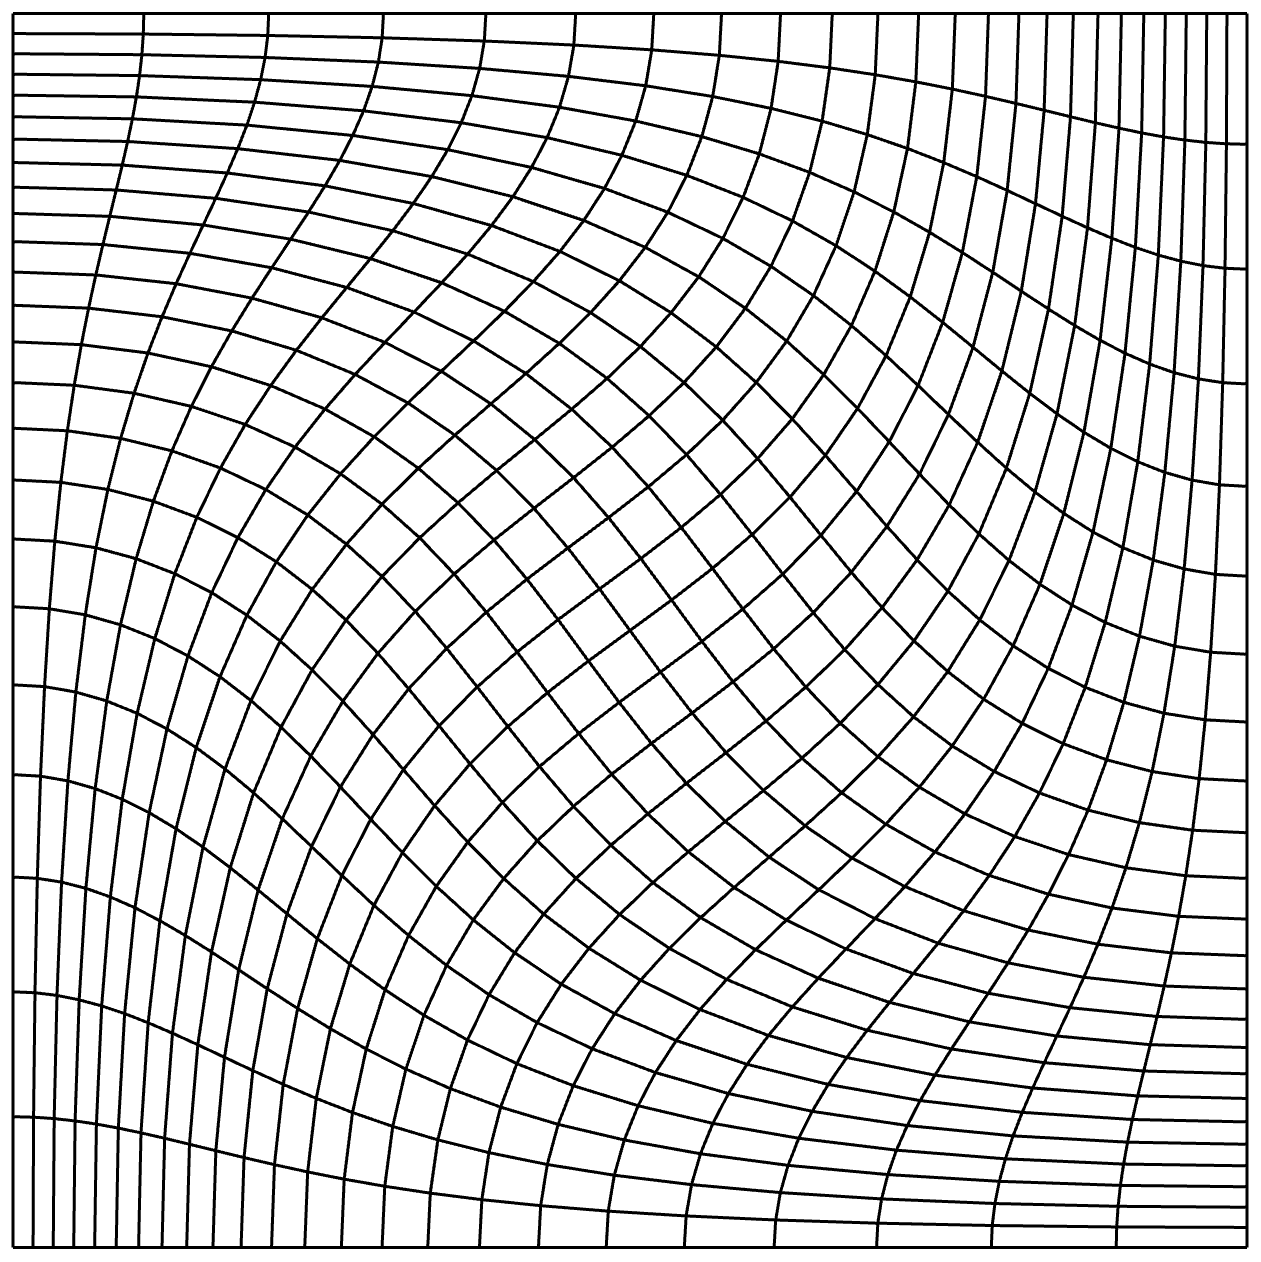
\includegraphics[width=.35\textwidth]{data/img/tgmesh0.3.png}
\caption{A depiction of a third-order mesh generated by distorting an orthogonal mesh according to the Taylor Green vortex. Refinements of this mesh are used in calculating the error with the method of manufactured solutions.}
\label{smm:tgmesh}
\end{figure}
We use refinements of a third-order mesh created by distorting an orthogonal mesh according to the velocity field of the Taylor Green vortex. This mesh distortion is generated by advecting the mesh control points with 
	\begin{equation}
		\x = \int_0^T \mat{v} \ud t \,,
	\end{equation}
where the final time $T=0.3\pi$ and 
	\begin{equation}
		\mat{v} = \begin{bmatrix} 
			\sin(x) \cos(y) \\ 
			-\cos(x) \sin(y) 
		\end{bmatrix}
	\end{equation}
is the analytic solution of the Taylor Green vortex. 300 forward Euler steps were used to advect the mesh. An example mesh is shown in Fig.~\ref{smm:tgmesh}. Logarithmic regression is used to fit the constant and order of accuracy according to 
	\begin{equation}
		E = C h^{\tilde{p}}
	\end{equation}
where $E$ is the error, $C$ the constant, and $\tilde{p}$ the order of accuracy. Four values of $h$ were used for each MMS problem considered in this section. 
The raw error values are provided in Appendix \ref{chap:mms_data}. 

Figure \ref{smm:mms_fig} shows the accuracy of the scalar flux on this MMS problem for a range of finite element polynomial orders. We see that all four methods have optimal $\mathcal{O}(h^{p+1})$ convergence for the scalar flux. As in the case for VEF, the IP and CG methods and RT and HRT methods have similar error behavior. 
% --- mms figures --- 
\begin{figure}
\centering
\begin{subfigure}{.4\textwidth}
	\centering
	\includegraphics[width=\textwidth]{figs/smm/mms.pdf}
	\caption{}
\end{subfigure}
\begin{subfigure}{.4\textwidth}
	\centering
	\includegraphics[width=\textwidth]{figs/smm/mms_1.pdf}
	\caption{}
\end{subfigure}
\begin{subfigure}{.4\textwidth}
	\centering
	\includegraphics[width=\textwidth]{figs/smm/mms_2.pdf}
	\caption{}
\end{subfigure}
\caption{Plots of the error in the scalar flux as the mesh is refined for (a) linear, (b) quadratic, and (c) cubic finite elements. A quadratically anisotropic MMS problem is used to ascertain the error.}
\label{smm:mms_fig}
\end{figure}

Next, we repeat the MMS problems from Section \ref{rtvef_sec:mms} used to probe the convergence of the current for the RT methods. Table \ref{smm:mms_diff} shows the error in the scalar flux, the error in the scalar flux when the exact solution is first projected onto a $Y_p$ grid function, and the error in the current on a diffusive MMS problem found by setting $\mat{\Theta} = 0$ in Eq.~\ref{smm:mms_psi}. It is observed that the two error values for the scalar flux converge with $\mathcal{O}(h^{p+1})$ and $\mathcal{O}(h^{p+2})$, respectively. In addition, the current converges with order $p+1$. On a diffusive problem such as this one, the SMM and VEF discretizations are equivalent. This is verified by the equivalent convergence rates and constants compared to the RT VEF methods in Table \ref{rtvef:mms_diff}. 
% --- MFEM MMS --- 
\begin{table}
\centering
\caption{Estimates of the order of accuracy and constant from an isotropic MMS test problem. The error in the scalar flux, the error in the scalar flux when the exact solution is first projected onto $Y_p$, and the error in the current are presented for each method over a range of values of $p$. Here, the VEF data are constant in space and thus are represented exactly.}
\label{smm:mms_diff}
\input{figs/smm/mms_diff}
\end{table}

Table \ref{smm:mms_table} repeats this test on the quadratically anisotropic MMS solution given in Eq.~\ref{smm:mms_psi} (i.e.~with $\mat{\Theta}$ as defined in Eq.~\ref{smm:mmsH}). Since the MMS solution is projected onto $Y_p$, it is expected that this problem can converge with a maximum of order $p+1$. This can be seen in the loss of superconvergence property. Here, both measures of the scalar flux error converge with $\mathcal{O}(h^{p+1})$. On this transport problem, the current convergence is also degraded. Both RT and HRT converge the current with $\mathcal{O}(h^p)$ for $p$ odd and $\mathcal{O}(h^{p+1/2})$ for $p$ even. Compared to Table \ref{rtvef:mms_same}, the SMM methods are no longer equivalent to their VEF counterparts. 
\begin{table}
\centering
\caption{Estimates of the order of accuracy and constant from a quadratically anisotropic MMS test problem. The error in the scalar flux, the error in the scalar flux when the exact solution is first projected onto $Y_p$, and the error in the current are presented for each method over a range of values of $p$. Here, the angular flux used to calculate the VEF data is represented with $Y_p$. Due to this, the maximum accuracy expected is order $p+1$. }
\label{smm:mms_table}
\input{figs/smm/vmms}
\end{table}

Finally, the MMS problem is repeated with the MMS angular flux projected onto the space $Y_{p+1}$ allowing a maximum accuracy of $\mathcal{O}(h^{p+2})$. The error measures are provided in Table \ref{smm:mms_elev}. Mixed finite element superconvergence is recovered as seen by $\|\varphi - \Pi \varphi_\text{ex}\|$ converging with order $p+2$ as in the diffusion case. In addition, the same behavior where the HRT method converges the current with order $p+1$ is observed with the RT method achieving $p+1$ only for $p$ even. 
\begin{table}
\centering
\caption{Estimates of the order of accuracy and constant from a quadratically anisotropic MMS test problem. The error in the scalar flux, the error in the scalar flux when the exact solution is first projected onto $Y_p$, and the error in the current are presented for each method over a range of values of $p$. Here, the angular flux used to calculate the VEF data is represented with $Y_{p+1}$. Due to this, the maximum accuracy expected is order $p+2$.}
\label{smm:mms_elev}
\input{figs/smm/mms_elev}
\end{table}

\subsection{Thick Diffusion Limit}
The performance of the SMM algorithm is investigated in the thick diffusion limit. The material data are set to 
	\begin{equation}
		\sigma_t = 1/\epsilon \,, \quad \sigma_a = \epsilon \,, \quad \sigma_s = 1/\epsilon - \epsilon\,, \quad q = \epsilon \,,
	\end{equation}
where $\epsilon \in (0,1]$ and the thick diffusion limit corresponds to $\epsilon \rightarrow 0$. We use two coarse meshes that do not resolve the mean free path to stress the convergence of the VEF method. The first is an orthogonal $8\times 8$ mesh with $\D = [0,1]^2$. The second is the triple point mesh shown in Fig.~\ref{smm:triple_point_mesh}, a third-order mesh generated with a Lagrangian hydrodynamics code where $\D = [0,7]\times [0,3]$. On the triple point mesh, the angular flux is only approximately inverted due to the lagging of reentrant faces and thus it is expected that convergence will degrade. In addition, highly distorted elements have poor approximation properties. We use Level Symmetric $S_4$ angular quadrature. The three methods are compared when $p=2$. The coupled transport-VEF system is solved with fixed-point iteration. 
% --- triple point mesh --- 
\begin{figure}
\centering
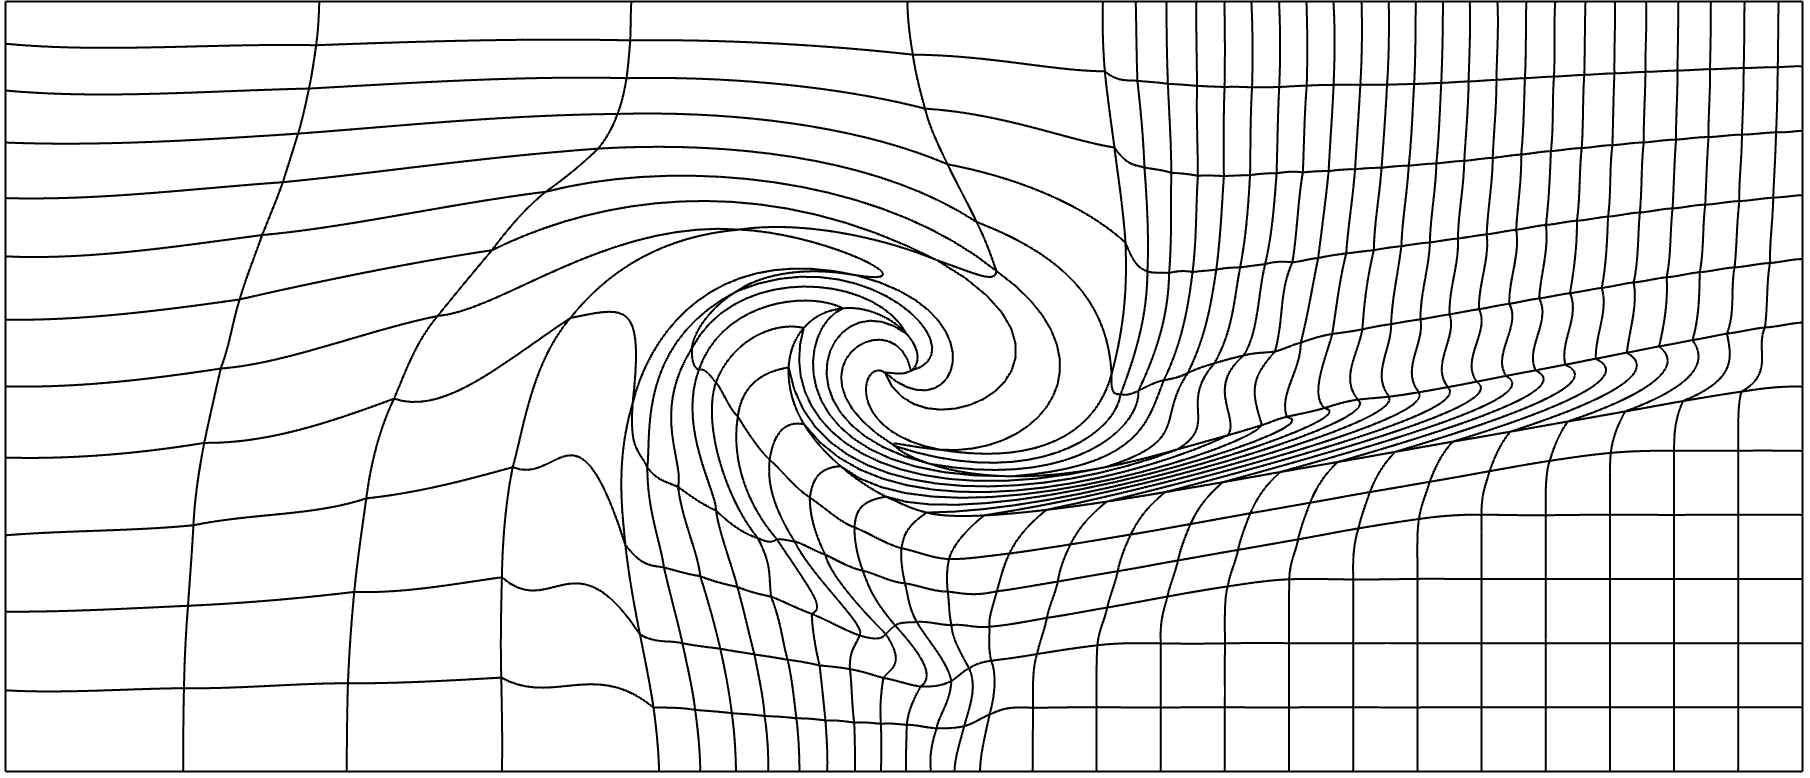
\includegraphics[width=.65\textwidth]{data/img/3point.png}
\caption{A depiction of the triple point mesh used to stress the VEF algorithms on a severely distorted, third-order mesh. This mesh was generated with a Lagrangian hydrodynamics simulation. }
\label{smm:triple_point_mesh}
\end{figure}

Table \ref{smm:tdl} shows the number of fixed-point iterations until convergence to a tolerance of $10^{-6}$ for each method on the orthogonal and triple point meshes. Rapid convergence is seen for all methods on both problems. 
The IP and CG and RT and HRT methods converged equivalently on the orthogonal mesh and nearly equivalently on the triple point mesh (RT converged in one fewer iterations for $\epsilon = 10^{-2}$). Compared to VEF, SMM required 1-3 more iterations on the orthogonal mesh. 
Lineouts of the 2D VEF scalar flux solutions for each method as $\epsilon \rightarrow 0$ are provided in Fig.~\ref{smm:eps_lineout} for the orthogonal mesh. In all cases, a non-trivial solution is found. 

% --- thick diffusion limit --- 
\begin{table}
\centering
\caption{The number of fixed-point iterations required for convergence as the thick diffusion limit parameter $\epsilon \rightarrow 0$. Convergence is tested on an orthogonal $8\times 8$ mesh and on the triple point mesh, a mesh with re-entrant faces. Due to the re-entrant faces, a partial transport sweep is used making convergence slower on the triple point mesh.}
\label{smm:tdl}
\input{figs/eps_table_smm}
\end{table}

% --- orthogonal lineouts --- 
\begin{figure}
\centering
\foreach \f in {figs/eps_lineout_ipsm.pdf,figs/eps_lineout_cgsm.pdf,figs/eps_lineout_rtsm.pdf,figs/eps_lineout_hrtsm.pdf}{
	\begin{subfigure}{.4\textwidth}
	\centering
	\includegraphics[width=\textwidth]{\f}
	\caption{}
	\end{subfigure}	
}
\caption{Lineouts of the 2D solution as $\epsilon\rightarrow 0$. The methods all converge to the asymptotic solution indicating they preserve the thick diffusion limit.}
\label{smm:eps_lineout}
\end{figure}

\subsection{Crooked Pipe} \label{smm_sec:cp}
We now show convergence in outer fixed-point iterations and inner preconditioned linear solver iterations on a more realistic, multi-material problem. The geometry and materials are shown in Fig.~\ref{smm:cp_diag}. The problem consists of two materials, the wall and the pipe, which have an 1000x difference in total interaction cross section. Time dependence is mocked by including artificial absorption and sources that correspond to backward Euler time integration. The time step is set so that $c\Delta t = 10^3$ and the initial condition is $\psi_0 = 10^{-4}$. The absorption and source are then $\sigma_a = 1/c\Delta t = 10^{-3} \si{\per\cm}$ and $q = \psi_0/c\Delta t = 10^{-1} \si{\per\cm\cubed\per\s\per\str}$. The boundary conditions are set so that isotropic inflow of magnitude $1/2\pi$ enters on the left entrance of the pipe. A Level Symmetric S$_{12}$ angular quadrature set is used. The quadratic programming negative flux fixup from \cite{YEE2020109696} is used inside the transport sweep to ensure positivity.  
% --- crooked pipe geometry --- 
\begin{figure}
\centering
\includegraphics[width=.65\textwidth]{figs/crooked_pipe.pdf}
\caption{The geometry, material data, and boundary conditions for the linearized crooked pipe problem. }
\label{smm:cp_diag}
\end{figure}

The outer fixed-point and inner linear iterative efficiency are shown by refining in $h$ and $p$ on an orthogonal mesh. Anderson acceleration with two Anderson vectors is used. The previous outer iteration's solution is used as an initial guess for the inner solver so that the initial guess becomes progressively more accurate as the outer iteration converges. The outer tolerance is $10^{-6}$ and the inner tolerance is $10^{-8}$. The IP, CG, and HRT methods used the conjugate gradient solver. CG and HRT are preconditioned with one AMG V-cycle. The IP method is preconditioned by the \gls{usc} preconditioner which uses one AMG V-cycle and one iteration of Jacobi smoothing. Finally, the RT method uses \gls{bicg} with a lower block triangular preconditioner that performs one iteration of Gauss-Seidel smoothing and one AMG V-cycle per iteration. 

Table \ref{smm:cp} shows the number of Anderson-accelerated fixed-point iterations to convergence and the maximum, minimum, and average number of inner iterations performed across all the outer iterations for each of the methods. The IP and CG methods and RT and HRT methods converged within one iteration of each other. The inner solvers were all scalable in both the mesh size and the polynomial order.  
% --- crooked pipe hp scaling --- 
\begin{table}
\centering
\caption{The number of outer Anderson-accelerated fixed-point iterations until convergence along with the maximum, minimum, and average numbers of inner linear iterations until convergence on the linearized crooked pipe problem. Two Anderson vectors were used. The previous outer iteration's solution was used as the initial guess for the inner iteration. }
\label{smm:cp}
\begin{adjustbox}{max width = \textwidth}
\input{figs/cp_smm}
\end{adjustbox}
\end{table}

\subsection{Weak Scaling} \label{smm_sec:weak}
Finally, we show that the methods scale in parallel. The parallel partitioning is such that there are $\approx\!\num{9000}$ VEF scalar flux unknowns per processor. The results were generated on 32 nodes of the \texttt{rztopaz} machine at LLNL which has two 18-core Intel Xeon E5-2695 CPUs per node. The materials and geometry from the crooked pipe in Section \ref{smm_sec:cp} are used. In Table \ref{smm:weak}, the number of linear iterations until convergence to a tolerance of $10^{-8}$ is shown when 1) a transport solve is used to compute the SMM correction sources and 2) the SMM correction sources are set to zero. The solvers are the same as those in Section \ref{smm_sec:cp}. We have used $p=2$. 
All the methods are scalable out to over a million elements and 1152 processors. Interestingly, the number of iterations for solving the SMM equations is increased compared to solving the corresponding diffusion problem. This suggests that the SMM correction sources make the inner solve more difficult. 
% --- weak scaling --- 
\begin{table}
\centering
\caption{A weak scaling study on the first iteration of the linearized crooked pipe problem. Inner linear iteration counts are compared when a parallel block Jacobi sweep is used to compute the SMM correction sources (SMM) and when the SMM sources are set to mock a radiation diffusion problem (Diffusion). }
\label{smm:weak}
\input{figs/smm/weak}
\end{table}

\end{document}